\chapter{Fixing flaws in economics}
\addcontentsline{toc}{chapterdescription}{Neoclassical economics is deeply flawed, because it is too much scientism, not enough science. We need to develop a general theory of economies that includes rational and irrational, thinking and feeling as complementary pairs. An economics that never assumes physics is irrelevant, satisfies thermodynamics, knows when a process is ergodic and when not, and works out of equilibrium. Such a general theory includes everything that works in the different, polarised approaches of today, is falsifiable, and most importantly predicts well what will happen. Like predicting the next crash. To get there we first need to understand the flaws.}
%\addcontentsline{toc}{chapterdescription}{\pagebreak}
\label{chapter:gen-th-economies-flaws}
%XXX Check all cross-references to this chapter


\begin{chapterquotation}
Science makes people reach selflessly for truth and objectivity; it teaches people to accept reality, with wonder and admiration, not to mention the deep awe and joy that the natural order of things brings to the true scientist. \\
\raggedleft\textemdash Lise Meitner\index{Meitner, Lise} 
\end{chapterquotation}


This final chapter of the economics part exposes the significant weaknesses in neoclassical economics\index{economics!neoclassical} and is written primarily for those of you really interested in economics, or in why we have taken such poor decisions over the past few decades. Neoclassical economic thinking, and its effects, are all around us, creating the life you are living, preventing the better life we could all be living.


At the end of the book  is an appendix for anyone wanting to dive deeper into a potential future alternative to current economic thinking, a speculative provocation pointing at a new concept of economics to navigate through our current turbulent time and build a better world.  




\section{Why didn't you see this coming?}
\ldots asked the Queen at the London School of Economics in 2008 to a group of the most senior economists in the UK. The 2008 crash, and how little has been improved since then\cite{guardian-groundhog-day}, is just one piece out of a wide range of evidence that neoclassical economics fails to accurately and reliably describe much of what actually happens in our economy. You can find much more in the excellent book \emph{Rethinking Capitalism}\cite{mazzucato-rethinking-capitalism} and the \emph{Global Minotaur}\cite{varoufakis-minotaur}. 


No wonder economists\index{economists}  are the kind of experts everyone is losing trust in\cite{wolf-economists-failed-experts}. Compare how economists\cite{keen-debunking} and physicists develop their theories. Physicists\index{physicists} always follow actuality (Section~\ref{section:reality-actuality}) where it leads them, turning hypotheses into evidence-based, validated theories, as in the quote from Lise Meitner above. And when something that they believed was a theory fails to predict, then it's evidence that it is no longer a theory, but at best an approximation, a phenomenological model, or, like believing the sun orbits the Earth, pure fantasy. 


Were neoclassical economics\index{economics!neoclassical} sufficiently robust and validated for a physicist to class it as a theory, every neoclassical economist would have predicted, by 2000, and with unambiguous clarity, that a crash was coming within the decade. That they didn’t is sufficient evidence that neoclassical economics falls short of the scientific criteria to become a theory.


Neoclassical economics is failing us, and whilst heterodox economics gives us a lot of value, we need even better. We urgently need a general theory of economies that describes precisely what is happening now and predicts reliably what will happen tomorrow. Including the impact on tomorrow of that prediction.


Getting there requires the characteristics of physicists like Einstein:\index{Einstein, Albert}  an openness to changing their mind, extreme stubbornness, and the humility to let go of both self-identity and beliefs in the face of data.


To catalyse a very different way of talking about what an economy is, I will use different metaphors, primarily Einstein's general relativity\index{general relativity}. A metaphor\index{metaphor}  is a \index{lens}  explicitly chosen to hide everything that is different, so that you can begin by focusing on everything useful that is similar. Once you reach the limit of similarity, the metaphor breaks down. So clearly a metaphor is only to be taken seriously, like any other lens, against a frame of reference\index{frames of reference}  of usefulness. 


As you read this chapter, please keep in mind the impossibility of capturing a metaphor in words. My words are no more than labels for concepts. You may use the same word to label a different concept, and different words to label the same concept. Please read into the concepts beyond the words.


Many jokes in physics start with the way physicists\index{physicists}  use impossible extremes to begin thinking. So if they are trying to understand the movement of a herd of cows being chased by a dog across a field, they will begin by saying: 
\begin{quote}
let's assume we have infinitely many 500kg spheres and one 20kg sphere.
\end{quote} 
They know that there are not infinitely many in the herd, that cows have legs and a body that is far from a sphere, but it's a good starting point to separate out what is complete rubbish from everything that might be true. 


Most importantly, a viable economic theory \index{economy!theory of}  will describe everything from one individual's personal economy all the way through to the global economy. Below are some key elements that need to be well described in any general theory.
\section{Decisions: rational or irrational?}
\index{decisions|(} 

\begin{quote}
Value is in the eye of the beholder. 
\end{quote}


The old saying, beauty is in the eye of the beholder, applies equally to all kinds of value\index{value}, and all kinds of decisions. It paraphrases an essence of this book: your reality, your meaning\hyp{}making is uniquely yours.


So what I see as rational, in my reality, you might see as irrational in yours. But your seeing my decision as irrational certainly does not make it an irrational decision in itself, it may only be \emph{not your rational}.


As you can see in Figure~\ref{table:rational-irrational}, the opposite of rational is not rational, and the opposite of irrational is not irrational. Sometimes this collapses from a two\-dimensional shape into just a straight line, and not rational is identical to irrational, but not always.


\begin{SCfigure}
%\begin{wrapfigure}{O}{0.55\textwidth}
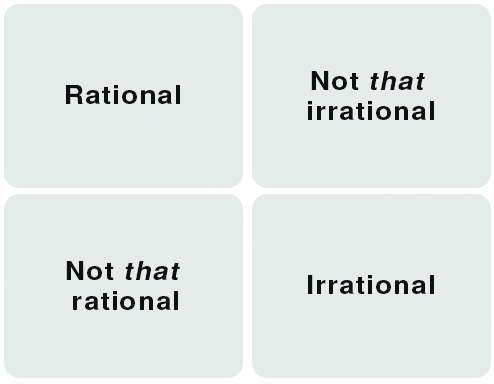
\includegraphics[width=0.45\textwidth]{./Images/Table-6_1}
\caption{Irrational is not always the opposite of rational.}
\label{table:rational-irrational}
%\end{wrapfigure}
\end{SCfigure}


Evaluating a decision as rational requires two components, not just one. 


\begin{enumerate}
\item The logic, or naked thinking process and outcome. 
\item The frame of reference used to evaluate the options processed by the naked thinking process. 
\end{enumerate}


So say something about what is rational if both the thinking process and the frame of reference are included in our theory. Then you might find that all decisions are rational; and those you evaluate as irrational are simply using a different meaning-making frame of reference, and / or a different thinking process?\index{decisions|)} 


\subsection{Thinking and feeling: a complementary pair}
This also makes it clear how to include feelings and emotions into the rational decision process. If you are scared of the dark, regardless of whether or not there is a physical threat hiding in the darkness, it is rational to avoid dark spaces, even if only to reduce your experience of the fear itself. Most of us have some set of dark spaces we avoid, at least non-physical spaces of ignorance and belief.


Neurobiology has shown that any human decision is a combination of thought and feeling. A decision is the feeling you have when one of the options you are choosing between fits into the frame of reference you're using to evaluate the options against; or in the language of Chapter~\ref{chapter:who-am-i-sense}, it's the feeling you have when your sense-making works. A decision is primarily a process of feeling, rather than one of thinking.


You may believe that thinking is thinking, feeling is feeling, and ne'er the twain shall meet.  
But if I am taking a decision\index{decisions},   I'm never just doing pure thinking without any other influence. How I feel at the time will be powerfully shaping how and what I'm thinking. If I'm feeling excited and confident, running fast from one decision to another, as somebody is on a trading floor, I will take a very different decision to the one I might take if I'm feeling deeply depressed because I've just heard bad news. Like the company I invested all of my client’s money in yesterday having just declared bankruptcy.


So I propose that we consider thinking and feeling to be a complementary pair\index{complementary pairs}  in the decision process, not opposites. Just like particles and waves in quantum physics.\index{physics!quantum} 


Then for me to understand your rationality\index{rationality}   leading you to take a very different decision to the one that I might take, I must work with both your thinking and your feelings during your decision as an inseparable complementary pair.\index{complementary pairs} 


\subsection{All decisions are rational}
None of us ever feels the force of gravity\index{gravity}. If you are sitting in a chair reading this book right now, take a moment to check what your body is feeling. I doubt you'll say, \emph{I feel gravity as a force throughout my body pulling me down}. Most likely you will say, \emph{I feel the chair pushing up}.


Einstein's general relativity (building on Section~\ref{section:applying-picasso-einstein}) describes everything we attribute to gravity in a way that aligns with your felt experience. General relativity\index{general relativity} came about because Einstein\index{Einstein, Albert}  asked himself whether there was any way that he could tell the difference between sitting on a chair in an elevator that was accelerating at $9.8m/s^2$ (the Earth’s gravitational acceleration) or sitting on a chair in an elevator stationary on the Earth’s surface.


He concluded that not being able to tell the difference was not due to his personal inability, but because there was actually no difference, there was no such thing as the force of gravity. It was a metaphor, useful in certain situations, like when we use the words sunrise and sunset even though we know it’s the Earth turning, not the sun rising and setting.


I propose that in a general theory of economies, the one reliable constant is that all decisions are rational, against whichever internal reality and frame of reference the entity taking the decision was using in the moment.


After all, at the exact moment each of us takes a decision, we judge that decision to be the best and most rational decision we can take according to the frame of reference we have available to us, the context we are in, including our feelings, the meaning we are making, and the options available to us. Our experienced reality of decisions\index{decisions}  is that they are rational in the moment at that point. Somewhat the same as we never experience the Earth pulling us down, rather we feel the chair pushing up.


Any judgement of a decision as irrational is someone else judging the decision, from their inner meaning-making, their thinking-feeling processes, at another point in space, and moment in time. Or it’s ourselves, some time later, when we are in a different context or emotional state, perhaps using different thinking-feeling processes and / or different meaning-making.


Einstein developed relativity by taking seriously the experimental data pointing at the crazy idea (in classical physics)\index{physics!classical}  that there was a universal speed limit: nothing could accelerate beyond the speed of light. 


We propose that every decision taken by every person is perfectly rational; and that  neoclassical economics\index{economics!neoclassical}  fails in part because it assumes that there is only one reality. Rather, what will build a fully viable general theory of economies\index{general theory of economies}  is taking every decision as perfectly rational within the decision-maker’s reality, according to their frame of reference, in the moment. 


This fits our experience of taking decisions\index{decisions}. How often do you deliberately, and in full awareness of what you are doing, choose irrationally? Very seldom. Even the phrase \emph{cut off their nose to spite their face} is rational in the moment, when spiting the face is more important than the costs. 


This is also comparable to how Einstein\index{Einstein, Albert}  developed his general theory of relativity\index{general relativity}  by realising that what we experience sitting in a chair is the actuality, not an artefact of our subjective experience. 


A final thought here, in preparation for the rest of the book: imagine how different your relationships with your colleagues, friends and family might become if you assumed that every action they took was fully rational; but within a different reality to yours? And so you then focused on exploring what their reality is, within which their action is rational? All of a sudden most of the emotional triggers disappear and are replaced by curiosity and exploration.








\section{Thermodynamic economics}
As a physicist (Graham), and having begun my university studies with physics (Jack), I find it inconceivable that the three laws of thermodynamics\footnote{(1) Energy is conserved in the universe, it can neither be created nor destroyed; (2) Total entropy (disorder) increases; and (3) Entropy approaches a constant at absolute zero, typically zero. } are not satisfied by all of economic thinking.\index{thermodynamics}  


I find it unfathomable that research into the thermodynamics of economies, (see Steve Keen\cite{keen-thermodynamic-economics}), has only recently begun.\index{Keen, Steve}  


\emph{No one has ever found anything anywhere in the universe that fails to satisfy the three laws of thermodynamics.}\index{thermodynamics} 


How on earth could anyone have imagined that anything in economics, a subset of human society in the benign physics of our planet, could be a valid description of how an economy\index{economy}  actually works while failing to satisfy them? 


If it did, physicists\index{physicists}  would be overjoyed at having thermodynamics, a theory that has withstood all attempts to falsify it for centuries, finally having its flaws exposed!


Thermodynamics\index{thermodynamics}  is so well tested because energy is one of the foundations of our universe and hence of our economy. Without available energy\footnote{Or what a physicist calls free energy, which is quite distinct from the absolute amount of energy in a system. Free energy\index{energy!free} is the amount of energy available to do work, i.e., to move something, and is in essence the temperature difference between the highest available temperature that energy can start from, and the lowest available temperature that it can degrade to. Some scientism is based on a confusion between free energy and absolute energy.}, there would be no life and no economy. Regardless of which theory of value you subscribe to, be it a utility theory, labour theory, or any other theory, you have no value without free energy.


You need energy to move physical objects from A to B, or to transform them from A into B. You need energy in your brain to make meaning of what is happening, to choose between A and B, and take a decision. Everything that economics is about begins with free energy and the laws of thermodynamics\index{thermodynamics}.  


A valid theory of economies, i.e., a general theory, must fully reflect thermodynamics.
\section{Ergodicity}
\index{ergodicity|(} 
\label{section:ergodicity}
Closely related to thermodynamics is ergodicity. Many business and investment failures occur because our economy is not ergodic. Yet most of economics assumes that it is. Something is ergodic when the average of a sequence of decisions is the same as the average of those decisions taken independently. 


The field of ergodic economics has recently emerged because a group of physicists showed how seldom ergodicity is a valid assumption in our economy\cite{buchanan-ergodicity, peters-ergodicity-economics}. As a physicist I (Graham) find it baffling that such a foundational assumption was not thoroughly tested decades ago. 


Ergodicity roughly means that there is no difference between the average of a thousand people taking a bet once each, and one person taking that bet a thousand times in succession.


For example\cite{peters-ergodicity-economics}, let's say you have \$1,000 in your wallet. I offer you a bet that if the coin you toss lands heads, I'll give you 50\% more (\$500); and if it lands tales, you give me 40\% (\$400) of what is in your wallet. If a thousand people repeat this once, on average each person will be \$50, or 0.05\%, better off. So neoclassical economists \index{economics!neoclassical} would say that the rational decision is to accept the bet.


However, if you repeat this bet long enough in succession, you will end up with nothing in your wallet. Which is unlikely to be rational in your reality, despite neoclassical economics deeming it rational!  And since the investment decisions of your pension fund are an equally non-ergodic sequence of bets over time, you ought to be personally concerned that the economy is treated as ergodic when it is not.


\begin{figure}
\centering
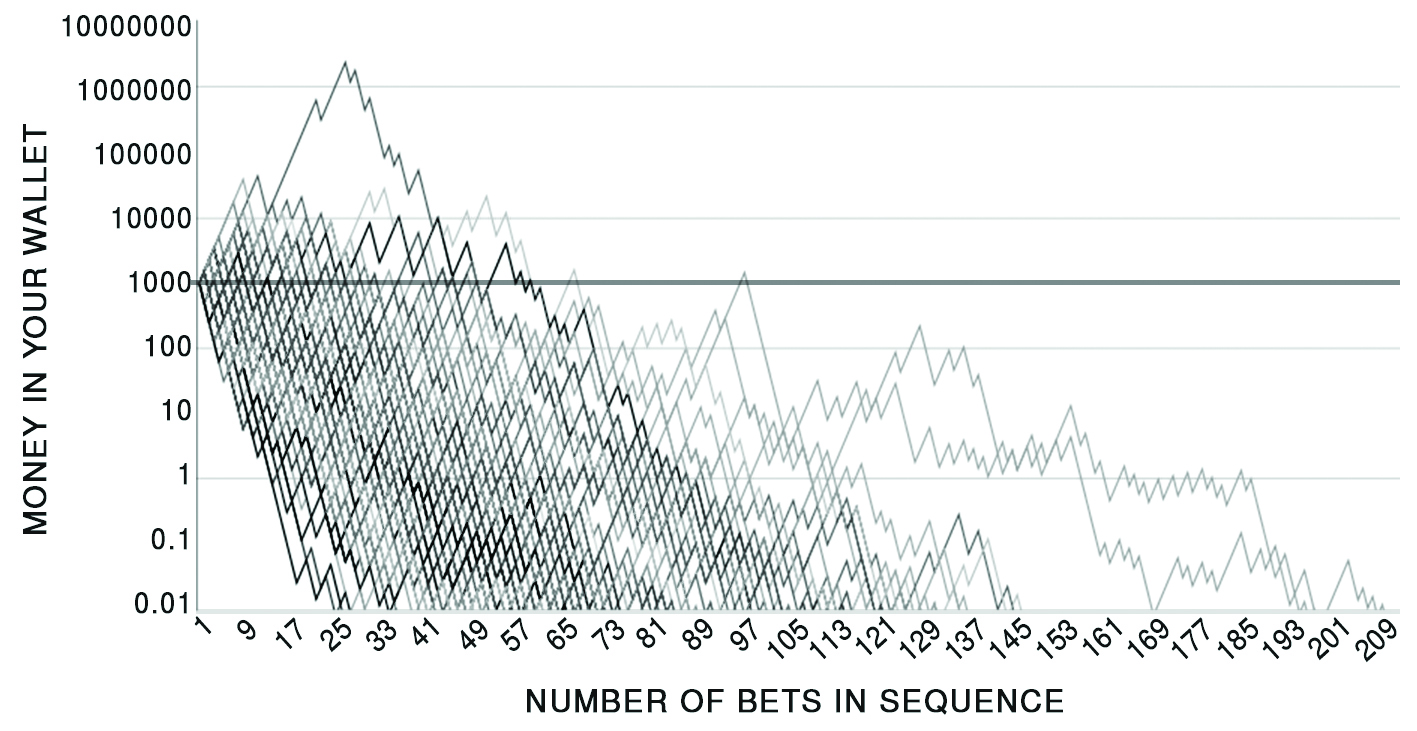
\includegraphics[width=0.90\textwidth]{./Images/bet-path-1c-cutoff}
\caption[Losing money long term even on a good bet.]{Looking at 100 people, each starting with 1000 in their wallet,  taking this decision 250 times in succession, everyone hits rock-bottom. In the graph, if you have less than 1c in your wallet, you can no longer bet, because you are unable to buy food and have starved to death. Only a few are tremendously lucky early on, making fabulous amounts of money.}
\label{fig:bet-path-1c-cutoff}
\end{figure}


This is just one of many examples where the rational decision in our economy\index{economy} is to refuse the bet because if you repeat it for long enough you are certain to lose money.


Much of economics\index{economics} incorrectly assumes ergodicity, i.e., that the gamble is positive over a long sequence. In fact, because the sequence does matter, on average you end up at a cumulative $-0.05\%$ worse off for each iteration.


To understand any individual's decision, even your own, you have to integrate every influencing event along that individual’s or your life path, which may well go back a number of generations. It's not for nothing that many ancient customs take into account seven generations. Think: \emph{I am my life path and the meaning-making stories that I have internalised because of that life path.} This means you are a process across time, not just you as you are now. (Read more in Section~\ref{sec:who-am-i}.)


This is also why so many ‘uneducated’ people are actually far better educated in how life works than graduates in business, economics, and all the other professions that have studied probability (those who Nassim Taleb\cite{taleb-skin}\index{Taleb, Nassim}  refers to as IYI\textemdash Intellectual Yet Idiot). Your life is \emph{one} sequence of many random events, not just many random events. What happens next often does depend on what happened before. In an extreme case, you can only win a huge amount if none of your previous bets has killed you. 


Be very careful of ergodicity in all of your life decisions, and be careful of economists when they look at life through their economic lens\index{lens} ; it may hide all non-ergodic aspects, and so be harmful to use. Investment decisions, e.g. how VCs choose to invest hoping for a Unicorn, may well be primarily luck (the single person surpassing a million in Figure~\ref{fig:bet-path-1c-cutoff}) in a non-ergodic economy. How ought you, as an investor, invest differently in a non-ergodic economy?


One consequence of this is that no description of economies based on everything being ergodic can be called a theory; it is only an approximation, because an economy is at most ergodic in a small subset of processes over short time spans.


We need a general theory of economies\index{general theory of economies}  that includes all ergodic and non-ergodic aspects of our economy. Simulating such a theory accurately requires a full path\hyp{}integral approach over at least one lifetime per person and a large enough number of people to accurately represent the entire population. Predicting the global economy next year will require something like a Markov Chain simulation of perhaps half a billion simulated people and their parents, taken through a path-integral from birth to today, with the full variety of life influences. 
\index{ergodicity|)} 
\section[Non-equilibrium: great shifts]{Non-equilibrium: great shifts in culture, energy, communication}
Neoclassical economics\index{economics!neoclassical}  only works in an equilibrium economy\cite{earl-econocracy}; and yet I doubt whether the global economy ever has been in equilibrium long enough for an assumption of equilibrium\index{equilibrium}  to be valid. The closest we get are locally approximate equilibria over short periods of time and small regions. Most of the time the economy is not in equilibrium.


A general theory of economies must work regardless of whether the economy is in a deep equilibrium or out of equilibrium.


It must work even in times of great change, such as for one of our current cultural and technical transformation, from a meaning making of burning fossil fuels\index{fossil fuels}  to make life convenient into one where burning fossil fuels is life-threatening.


A useful general theory of economies must also be able to tell the difference between bubbles\cite{carlin-macroeconomics}\index{Carlin, Wendy}  and the emergence of new paradigms of value. A bubble is where the price and / or supply increases as demand increases, but the meaning-making stories are fantasy, with little grounding in actuality. By new paradigms of value, I mean that a business concept that previously had no or negligible value becomes, over time, a business concept with high value in actuality.


Both are about as far from equilibrium as you can get, yet have quite different outcomes that the theory must predict from the early signals. 


To be useful, such a general theory of economies must describe the entire progression, from the first individual who comes up with something that later turns into either a bubble or a new value paradigm, through to the end state of either the bubble collapsing or the new value paradigm establishing itself.






\section{Competition and collaboration}
One assumption of neoclassical economics\index{economics!neoclassical}  is that perfect competition is desirable as the ideal way of distributing resources. Perfect competition\index{competition!perfect}  is a bit like the spherical cows example above\textemdash it assumes there are infinitely many producers and consumers, all of them identical, independent and so small that none ever influences the other.


If you look around you today, this is far from true. 


\begin{itemize}
\item We have some supermassive producers and consumers, akin to white dwarfs or black holes\index{black hole}  in general relativity\index{general relativity}.  
\item We have memes that sweep through society, aligning and freezing people's opinions into for or against, just as the climate emergency \index{climate!emergency} meme is now. 
\item And individual people talk to each other, reflect on what they experienced yesterday, and then change their opinions.
\end{itemize}


Any good theory of economies needs to work across the full range, from complete independence to complete alignment, from perfect competition through to all opposites of perfect competition. A general theory of economies based on the uniqueness of each individual’s experienced reality and the relativity of our respective unique realities may be such a theory.


Clearly the extreme points of 0\% or 100\% perfect competition\index{competition!perfect}  only occur for fleeting moments, much like the pendulum of a grandfather clock is only stationary for a fleeting moment at the top left and top right of its swing. Our economy is in constant dynamic motion across the space defined by the complementary pair of competition\index{competition}  and collaboration\index{collaboration}, just as Darwin\index{Darwin, Charles}  saw in nature\index{nature}. One issue in economics today is that competition and collaboration are seen as mutually exclusive opposites, rather than as one inseparable complementary pair, \index{complementary pairs} where the economy\index{economy}  always has and needs a mixture of both to be functional.


\begin{longstoryblock}
You can see this in how Graham and Jack have worked with each other on this book. It is the outcome of competition and collaboration as one single complementary pair. If you'd been a fly on the wall watching us right now as we discussed writing this chapter (and neither of us had swatted you), you would have seen that there was competition between the concepts each of us saw. The difference in how each of us saw these concepts comes from our different histories, our different knowledge and our different perspectives on the world. The conflict enabled us to see better what it was that the book needed to have, and the collaboration around producing the best possible book that the two of us could have written. 


So even just between the two of us, and within the narrow space of writing this book, we have an economy based on the complementary pair of collaboration and competition. And a general theory of economies needs to accurately describe exactly what Jack and I have experienced as we moved half-formed thoughts and concepts through a forming process into the final fully-formed words on the page, by doing work on the thoughts and concepts. By taking decisions, making choices, using our own decision spacetime to tell us how to move and work on the resources of our thoughts and concepts, to finally produce the paragraph you are now reading. 
\end{longstoryblock}






\section{Value is relative}
\index{value|(} 


Neoclassical economists approach to value, pricing, and rent is a root cause of much of today’s mess\cite{mazzucato-value-everything}.\index{Mazzucato, Mariana}  It, and using GDP\index{Gross Domestic Product} as a measure, is flawed. Activities can add to GDP even though they destroy total wealth; for example, an oil spill can add to GDP, even though it killed vast swathes of our life-support systems on the planet. 


Two approaches in economics to value are that it is either 1) intrinsic, or 2) based on the value of the labour that went into making it. 


\begin{longstoryblock}
“What is this book’s value?” we asked each other whilst writing this chapter. 


We concluded that it is neither in the book nor in the labour, and yet it is in the book and in the labour, and in both together. Paradox and complementary pairing strike again. The value depends on your frame of reference and how you use the book; whether you read it, light a fire with it, or as rubbish for recycling. 


The value changes over time, as each reader gets deeper and deeper into converting the book into insights and actions that are valuable to them (perhaps uniquely to them). The value is clearly not only in the labour of, and financial costs to Jack and myself in, creating the book’s concepts, nor only in crafting the words, although that is certainly an important contributor to the value that some readers perceive in it.


The value clearly lies in your individual meaning-making, and in how larger groups of people collectively make meaning and thereby create value and an appropriate pricing for this book. It might be a brilliant book that never gets sufficiently well known to sell widely, or it may be abysmal and filled with rubbish but just happens to catch a meme as it emerges and goes viral. The value in each case is neither in the book’s utility, nor its labour, and yet both are essential parts of creating the value for you. 
\end{longstoryblock}


In the general theory of economies, \emph{value is always in the eye of the beholder}. Value is always attributed by the beholder, according to their meaning-making frame of reference, including their emotional state, at some point in time, and including their beliefs about any relevant intrinsic, utility, labour, etc. value. 


So a general theory of economies\index{general theory of economies}  must give us a mechanism to take all value drivers today\cite{mason-post-capitalism}\index{Mason, Paul}  and bring them all together into the final value that’s used to take a decision.


As Jack and his co-authors wrote in their pluralist economics textbook\cite{reardon-introducing},\index{Introducing a New Economics: Pluralist,Sustainable, and Progressive}  the meaning and origin of value in economics has always been one of the most contentious areas in economics\index{economics}.  


The general theory of economies must provide a framework to bring them all together in a way where each complements the other, and where it becomes clear in each situation which value driver plays which role; if one is dominant, so it's a good enough local approximation to calculate as if it is the only driver of value; or if all are significant, so you cannot make your life easier by using a local approximation; and how to then include them all to represent the value used to take a decision.


I believe that the underlying reason why we have not yet such a general theory of economies lies in the human dimension described in Part~\ref{part:you}. Too few economists have developed the fluidity in the 28 thought forms,\index{thought forms (28)}  and the requisite meaning-making stage of development, to be easily able to take distance from their own beliefs, to hold opposing concepts as simultaneously true, and coordinate multiple open systems. 




\section{Externalities and conflict}
\index{externalities|(} 
An externality is one of the trickier aspects of economics\index{economics},   so in case you’ve not yet encountered the concept, here’s a quick example. You’ve gone shopping, and choose to save a bit of money by buying fruit reduced to 50\%. That night you and your partner have an upset stomach, get no sleep, and both of you lose a day’s income the following day. Your health costs were an externality in your decision to buy the lower-cost fruit because you excluded those costs and risks from your economic decision. 


Often people think externalities are only negative\index{externalities!negative}, but they can also be positive.\index{externalities!positive}  Examples of both positive and negative externalities, well-known in business theory and neoclassical economics,\index{economics!neoclassical}  are the exclusion of essential elements of our natural and social environment: the costs created by air pollution damaging our health (negative); or the benefits to society of investing in education (positive), are usually excluded\textemdash labelled as “external to the theory”, even though everyone recognises that these “externalities” are central to the system working in the first place! Heavy investment in education is a big driver of positive externalities in social, economic, and business success a couple of decades later.


We’re facing the global crises of today because neoclassical economics mistakenly believes you can exclude core elements of the whole system. 


On any finite world, in any closed system, there cannot in actuality be any externalities, and any compartmentalising approach yielding externalities fails the first test for becoming a useful theory. And so in a general theory of economies there are no externalities: all elements and their impacts across the whole are part of a general theory.


Take our climate emergency, \index{climate!emergency} for example. By treating the insulating blanket of our atmosphere as an externality, our economic decisions fail to take into account the steady increase in insulation caused by increasing pollution with carbon dioxide. This is causing less energy to flow out than flows in, which is steadily raising the temperature, which will keep rising until the increased driving force from a higher temperature forces more energy out through the more insulating atmosphere, and so re-establishes thermodynamic equilibrium. 


We've got into this mess in part because economics\index{economics}  has tried to simplify itself by neglecting thermodynamics and making invalid assumptions of ergodicity, and of externalities where there are none, and more. There would be far less risk of the kind of climate emergency we are now in, had we had a general theory of economies 50 years ago. High time we develop one! (Ironically, in the attempt to become more scientific, much of neoclassical economics\index{economics!neoclassical}  has become more scientism.)\index{scientism} 


Another deep cause of our mess lies in how economics includes (or doesn’t) conflict and how economists approach conflict between practitioners. The general theory of economies\index{general theory of economies}  picks up on a theme running through this book: the beneficial, generative role of conflict and tension. The conflict\index{conflict}  between different stakeholders\index{stake}  in a business, such as the conflict\index{conflict}  between labour and management, is necessary for its structural integrity and adds value.


Conflict shapes choices in a marketplace, is essential, and has potential downsides. The conflict between buyer and seller generates the structural integrity of a market. But, a buyer who is small, perhaps only 10 years old, physically quite weak, and with a set of meaning-making stories that are harmony-seeking, negotiating a price with a large, powerfully built, middle-aged seller with psychopathic tendencies will yield a different outcome to the same two people, but swapping the role of buyer and seller.  


To truly capture a theory of value that reflects society and any economy, it's vitally important that we know if value is ergodic or not, and if not always use a path integral across each individual's life segment. Price and value are usually far from ergodic because conflict is not ergodic\index{ergodicity}.  What you value depends on your history, the path your life has travelled along.


Neoclassical economics\index{economics!neoclassical}  sweeps under the rug\cite{dowd-capitalism}\index{Dowd, Douglas} the inherent value of conflict,\index{conflict}  and the consequences for each person’s inner, unique, rational theory of value. So, neglecting how humans thrive, a zero-conflict equilibrium economy becomes the ideal to strive for.


This is mistakenly treating an extreme simplification, which may or may not be useful to get a rough idea of how an economy works, as if it is the ideal actuality\cite{thurow-dangerous}. Early neoclassical economists made simplifying approximations in order to be able to calculate anything, as they lacked computers and today’s understanding of adult development and meaning making. 


Tension and conflict,\index{conflict}  (at all six levels in Section~\ref{section:harnessing-conflict-intro}, Page~\pageref{section:harnessing-conflict-intro}) are two of the most intractable aspects of human nature and the social sciences, and quite obviously two of the most challenging elements to include in any general theory of economies. They are also essential for life, including any economy, to function: tension and conflict are just an expression of some difference, and differences are the precursor of all the value flows that make an economy.\index{externalities|)} 




\section{The role of freedom and property}
There has long been an imprecise grasp of the central role of freedom\index{freedom}  and property\index{property} in an economy.\index{economy}  In a general theory of economies\index{general theory of economies}  we must have a formulation to precisely grasp the consequences of freedom and property in an economy.


And well done if you have already recognised that we wrote role, singular, as we see freedom and property as a complementary pair\index{complementary pairs},   not as opposites! Freedom\index{freedom}  we define as the freedom to be yourself, including the freedom to take your own decisions according to your reality. This includes the possibility that your self is nebulous, changing, or even porous. Property\index{property}  we define as having the sole decision authority over something. As with any complementary pair, property and freedom are related to each other.


Freedom and property each label an entire library of contested stories of what each is, or even ought to be. For example, freedom in the US is primarily taken to be the freedom of the individual to choose and strive, seldom taking into account the impact of the individual's current environment, and past life path, on the possibility of that choice and that striving leading anywhere.


On the other hand, freedom in China is more anchored in the freedom of the community to remain harmoniously together as a community, which leads to less freedom of individual choice and speech.


Any general theory of economies \index{general theory of economies} must represent all kinds of freedoms across the full range from 0\% to 10\% and predict the characteristics of an economy as freedom slowly moves from one point to another.


More or less freedom is not necessarily better, for all definitions of better. A young child's preference for a large bowl of sweet chocolate ice cream, instead of a bowl of Brussels sprouts coated in a light flavouring of butter and nutmeg, is one that, most of the time, is not better for the child's development into a healthy adult. It may well be better for the parent to rest by having a peaceful child; though the sugar rush may make it a suboptimal choice an hour later.


Equally, more or less ownership is not necessarily better.


Each amount of freedom, and each amount of ownership, has an impact. What is important is that anything less than 100\% freedom to take the exact decision of your own reality will lead to internal conflict and stress. That stress will then have a recursive, iterative effect on the meaning making you actually use to take your next decisions\footnote{Autocorrect in the Google Docs that I'm typing this in, is constantly suggesting that I correct my usage of “take a decision” to the more US usage “make a decision”. I have chosen to keep with the more English usage, take a decision, because it reflects the way that a decision is a choice between two or more options, and all you can do is take one option and leave the others. The making comes later, after you have taken the decision, when you turn the decision into action and results.}.


For example, think of the slaves who were once property and were then declared to no longer be property. This step from being 100\% property to 0\% property was not the same as having complete freedom to move. Because of their entire life path, they were not free to move in socio-economic space in the same way that somebody who had never been a slave was. Elements of these hidden, systemic losses of full freedom can remain in many individual’s experienced reality for generations, even if not visible in actuality.


We are all becoming more aware of these hidden, systemic consequences of life path over generations, as seen in the rise of Black Lives Matter, and many other movements aimed at addressing deeply embedded systemic unfairness.


Because freedom\index{freedom}  and property\index{freedom} are complementary pairs,\index{complementary pairs}  and each changes as you move from the scale of individual through families, small communities, regional communities, nation states, and on to larger groupings of nations and the entire planet, there are boundaries on freedom and property within any specific layer imposed by the layers above and below. All this is part of a general theory of economies\index{general theory of economies}. 






\section{The need for free companies}
The free company\index{company!free} (e.g., the FairShares Commons) has a competitive edge in many economies because the freedom enables the company both to take the best possible decision and be held fully accountability for the outcome.


If a company is not free, but is subject to forces (anything that can force a company to take a specific choice), or even property, somewhat like an individual being a slave, then they will make a forced choice.


Sometimes such a forced choice may well be the best one. For example, a company may have a decision-making board lacking the long-term perspective needed to make a wise decision, like an immature child choosing to eat chocolate ice cream instead of Brussels sprouts. Then the force of a regulation may be needed.


Or it may be a harmful one, such as where a company is forced to sacrifice the long-term interests of society and the environment by investors forcing higher short-term returns. 


If an individual is forced to use a frame of reference for a decision that’s different to the right one in their inner reality, they will experience internal stress. 


So too will a business. 


And as soon as the stresses imposed on that business by the gap between its natural decision and the one it is forced to take are bigger than the strength of the business’s structures to hold everything together, it will collapse or explode.


I suspect that research will show that a number of business failures are due to this. Nokia immediately springs to mind as an example.






In a free company, such as the FairShares Commons\index{FairShares Commons}  described in this book, the business has a much wider range of information included in its decision processes because every stakeholder has a voice and vote in the general meetings. Also, because the business is free to choose according to its own path, and is not constrained by the opinions and needs of the most powerful investors, it has far more room to take decisions that keep the business optimised for all, and within a viable level of stress.


So I see the Free FairShares Commons, or similar free incorporation approaches, as a necessary building block, in combination with other elements, for constructing a healthily thriving economy that does the job of provisioning for all.


Keep in mind that this does not mean a complete absence of any kind of property. A Free FairShares Commons company may well own buildings, land, other resources, and even fully owned subsidiary legal entities. After all, even though you’re a free human, your fingers, eyes and ears are not free to do their own thing. And if your heart starts doing its own thing, we call it a heart attack and rush you to hospital.


Only a free company, like the FairShares Commons, can always take a locally rational, natural decision and therefore be held accountable for the consequences. Failing that, the company will take a non-rational, forced decision; forced by whoever has a disproportionate amount of power over the non-free company, most likely harming the company, the environment, and many stakeholders. 


And how often do those with high levels of power force a company to take a decision that is rational for them\textemdash the investor, or founder, or head of the family\textemdash but is not rational for the company and ends up killing it?


You can read our current thoughts, that we hope will provide a useful catalyst for developing a general theory, in the appendix at the end of the book.


I believe that the economy as a whole can thrive best if each company is free to take the decision according to its natural path, which by definition includes all stakeholders’ perspectives, including future stakeholders that may need to bear the consequences of decisions. That replaces almost all regulation, in an even better way, as the right choice is informed by all affected by it. This requires everything described in this book about developing ourselves and organisations.